\documentclass[border=10pt]{standalone}
\usepackage{tikz}
\usetikzlibrary{arrows.meta, positioning, calc, fit}

\begin{document}
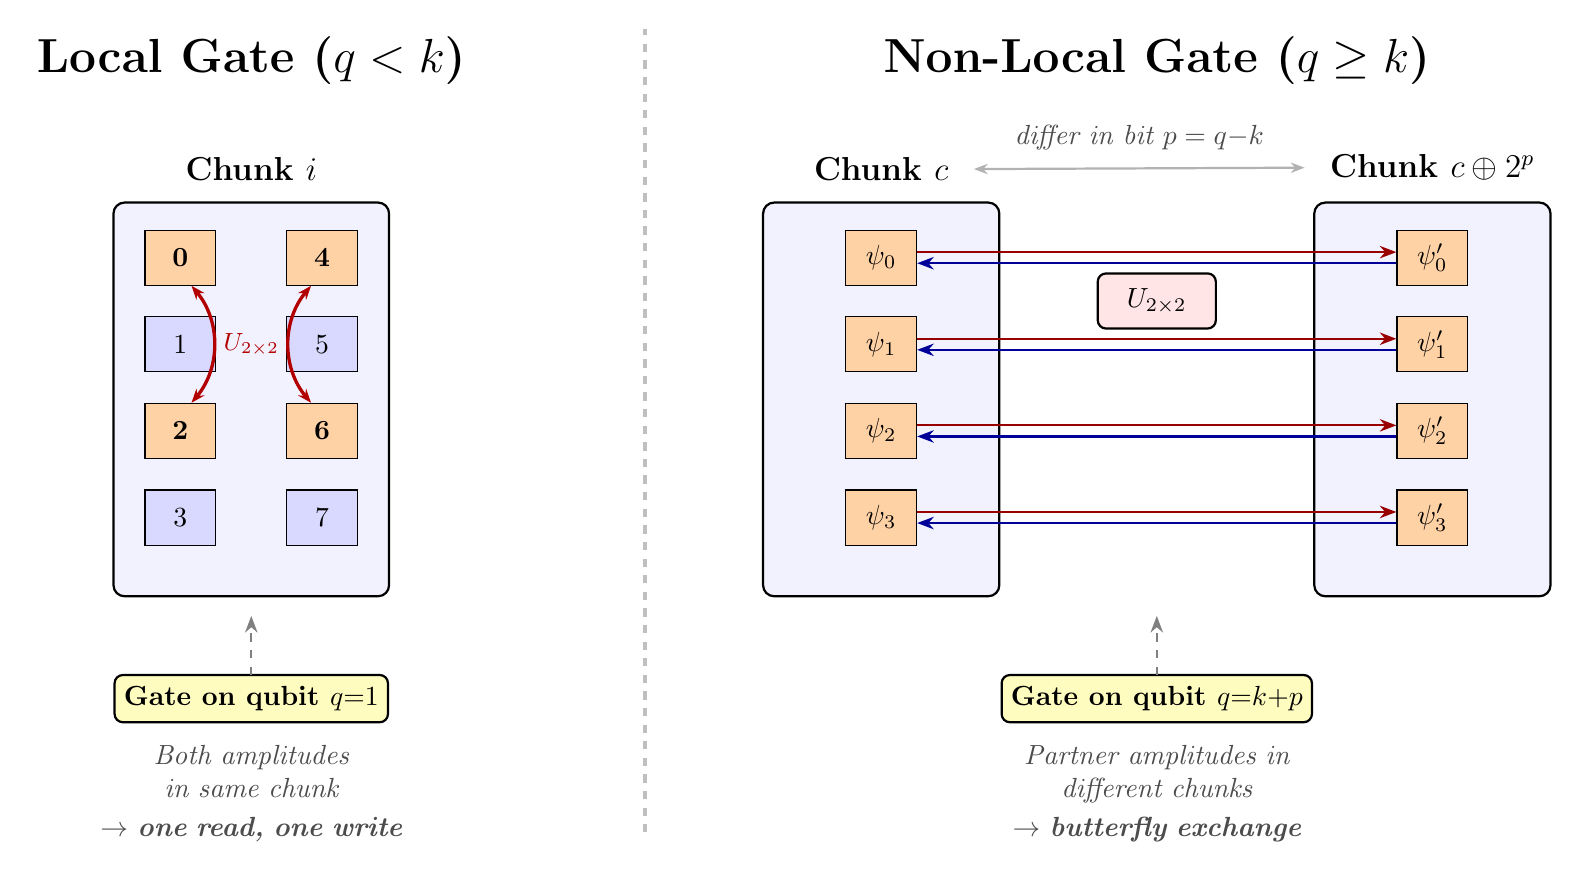
\begin{tikzpicture}[
    chunk/.style={draw, thick, minimum width=3.5cm, minimum height=5cm,
                  rounded corners=4pt, fill=blue!5},
    amp/.style={draw, thin, minimum width=0.9cm, minimum height=0.7cm,
                fill=blue!15, inner sep=0pt, font=\normalsize},
    amp_hi/.style={amp, fill=orange!35},
    gate_label/.style={draw, thick, fill=yellow!25, rounded corners=3pt,
                 minimum width=2cm, minimum height=0.6cm, font=\normalsize\bfseries},
    myarrow/.style={-{Stealth[length=6pt]}, thick},
    note/.style={font=\normalsize\itshape, text=gray!60!black},
    heading/.style={font=\LARGE\bfseries},
]

% ===================== TITLES =====================
\node[heading] at (3, 7.8) {Local Gate ($q < k$)};
\node[heading] at (14.5, 7.8) {Non-Local Gate ($q \geq k$)};

% ===================== LEFT: LOCAL GATE =====================

\node[chunk] (LC) at (3, 3.5) {};
\node[font=\large\bfseries, above=4pt of LC.north] {Chunk $i$};

% Amplitudes: two columns, 4 rows
\foreach \r/\v in {0/0, 1/1, 2/2, 3/3} {
    \node[amp] (L\v) at ($(LC.center)+(-0.9, 1.8 - \r*1.1)$) {\v};
}
\foreach \r/\v in {0/4, 1/5, 2/6, 3/7} {
    \node[amp] (L\v) at ($(LC.center)+(0.9, 1.8 - \r*1.1)$) {\v};
}

% Highlight paired amplitudes for qubit 1: (0,2), (4,6)
\node[amp_hi] at (L0) {\textbf{0}};
\node[amp_hi] at (L2) {\textbf{2}};
\node[amp_hi] at (L4) {\textbf{4}};
\node[amp_hi] at (L6) {\textbf{6}};

% Pair arrows — double-headed (data flows both ways), U label centered
\draw[{Stealth[length=5pt]}-{Stealth[length=5pt]}, red!70!black, very thick]
    ([xshift=4pt]L0.south) to[bend left=40]
    ([xshift=4pt]L2.north);
\draw[{Stealth[length=5pt]}-{Stealth[length=5pt]}, red!70!black, very thick]
    ([xshift=-4pt]L4.south) to[bend right=40]
    ([xshift=-4pt]L6.north);
\node[font=\small, red!70!black] at ($(LC.center)+(0, 0.7)$) {$U_{2\times 2}$};

% Gate label — close to chunk
\node[gate_label] at (3, -0.3) {Gate on qubit $q{=}1$};
\draw[myarrow, dashed, gray] (3, 0.0) -- (3, 0.75);

% Annotation
\node[note, text width=4.5cm, align=center] at (3, -1.5)
    {Both amplitudes in same chunk\\[2pt]$\rightarrow$ \textbf{one read, one write}};

% ===================== DIVIDER =====================
\draw[gray!50, dashed, very thick] (8, -2) -- (8, 8.2);

% ===================== RIGHT: NON-LOCAL GATE =====================

% Two chunks, well separated
\node[chunk, minimum width=3cm] (RA) at (11, 3.5) {};
\node[chunk, minimum width=3cm] (RB) at (18, 3.5) {};

\node[font=\large\bfseries, above=4pt of RA.north] (titleA) {Chunk $c$};
\node[font=\large\bfseries, above=4pt of RB.north] (titleB) {Chunk $c \oplus 2^p$};

% "differ in bit" — arrow spanning between chunk titles
\draw[{Stealth[length=5pt]}-{Stealth[length=5pt]}, gray!60, thick]
    (titleA.east) ++(0.2, 0) -- ($(titleB.west) + (-0.2, 0)$)
    node[midway, above=3pt, font=\normalsize\itshape, text=gray!60!black]
    {differ in bit $p = q{-}k$};

% Amplitudes in chunk A
\foreach \r/\v in {0/0, 1/1, 2/2, 3/3} {
    \node[amp_hi] (A\v) at ($(RA.center)+(0, 1.8 - \r*1.1)$) {$\psi_{\v}$};
}

% Amplitudes in chunk B
\foreach \r in {0, 1, 2, 3} {
    \node[amp_hi] (B\r) at ($(RB.center)+(0, 1.8 - \r*1.1)$) {$\psi_{\r}'$};
}

% Butterfly arrows — red right, blue left (offset to avoid overlap)
\foreach \r in {0, 1, 2, 3} {
    \draw[myarrow, red!60!black, thick]
        ([yshift=2pt]A\r.east) -- ([yshift=2pt]B\r.west);
    \draw[myarrow, blue!60!black, thick]
        ([yshift=-2pt]B\r.west) -- ([yshift=-2pt]A\r.east);
}

% U label centered — between psi0 and psi1 rows
\node[draw, thick, fill=red!10, rounded corners=3pt,
      minimum width=1.5cm, minimum height=0.7cm,
      font=\normalsize\bfseries] at (14.5, 4.75) {$U_{2\times 2}$};

% Gate label
\node[gate_label] at (14.5, -0.3) {Gate on qubit $q{=}k{+}p$};
\draw[myarrow, dashed, gray] (14.5, 0.0) -- (14.5, 0.75);

% Annotation
\node[note, text width=4.5cm, align=center] at (14.5, -1.5)
    {Partner amplitudes in\\different chunks\\[2pt]$\rightarrow$ \textbf{butterfly exchange}};

\end{tikzpicture}
\end{document}
